% Contributions are much appreciated, in order to contribute to this project, head over to this repository:
% https://github.com/bshramin/uofa-eng-assignment

\documentclass[11pt,letterpaper]{article}
\textwidth 6.5in
\textheight 9.in
\oddsidemargin 0in
\headheight 0in
\usepackage{graphicx}
\usepackage{fancybox}
\usepackage[utf8]{inputenc}
\usepackage{epsfig,graphicx}
\usepackage{multicol,pst-plot}
\usepackage{pstricks}
\usepackage{amsmath}
\usepackage{amsfonts}
\usepackage{amssymb}
\usepackage{eucal}
\usepackage[left=2cm,right=2cm,top=2cm,bottom=2cm]{geometry}
\usepackage{esvect}
\pagestyle{empty}
\DeclareMathOperator{\tr}{Tr}
\newcommand*{\op}[1]{\check{\mathbf#1}}
\newcommand{\bra}[1]{\langle #1 |}
\newcommand{\ket}[1]{| #1 \rangle}
\newcommand{\braket}[2]{\langle #1 | #2 \rangle}
\newcommand{\mean}[1]{\langle #1 \rangle}
\newcommand{\opvec}[1]{\check{\vec #1}}
\renewcommand{\sp}[1]{$${\begin{split}#1\end{split}}$$}

\usepackage{lipsum}

\usepackage{listings}
\usepackage{color}
\usepackage{wrapfig}
\usepackage[shortlabels]{enumitem}

\definecolor{codegreen}{rgb}{0,0.6,0}
\definecolor{codegray}{rgb}{0.5,0.5,0.5}
\definecolor{codepurple}{rgb}{0.58,0,0.82}
\definecolor{backcolour}{rgb}{0.95,0.95,0.92}

\lstdefinestyle{mystyle}{
	backgroundcolor=\color{backcolour},   
	commentstyle=\color{codegreen},
	keywordstyle=\color{magenta},
	numberstyle=\tiny\color{codegray},
	stringstyle=\color{codepurple},
	basicstyle=\footnotesize,
	breakatwhitespace=false,         
	breaklines=true,                 
	captionpos=b,                    
	keepspaces=true,                 
	numbers=left,                    
	numbersep=5pt,                  
	showspaces=false,                
	showstringspaces=false,
	showtabs=false,                  
	tabsize=2
}

\lstset{style=mystyle}

\begin{document}
\pagestyle{plain}

\begin{flushleft}
Estudiante: Fabio Quimbay\\
Email: fabio.quimbay883@comunidadunir.net\\
Profesor: Miguel Ángel Cabeza\\
Fecha: Noviembre 12 de 2022\\
\end{flushleft}

\begin{flushright}\vspace{-20mm}

\includegraphics[height=2cm]{logo.png}
\end{flushright}
 
\begin{center}\vspace{0cm}
\textbf{\large PER5786 2022-2023  Física 1 (GFI) - PER5786 2022-2023}\\
 Tema 3 - Movimientos elementales
\end{center}

 
\rule{\linewidth}{0.1mm}
%%%%%%%%%%%%%%%%%%%%%%%%%%%%%%%%%%%%%%%%%%%%%%%%%%%%%%%%%%%%%%%%%%%%%%%%

\bigskip
\bigskip

%%%%%%%%%%%%%%%%%%%%
\textbf{Problema propuesto 6}\\

\begin{enumerate}
  \item Sabiendo que la tierra tarda aprox. 24 horas en dar un giro completo, calcula su velocidad angular de giro, $\omega$.
  \item Sabiendo que el radio terrestre es $r = 6378.137\,km$, calcula el módulo de la velocidad lineal  de un punto A sobre la superficie terrestre en función de su latitud $\lambda$.
  \item Calcula la aceleración centrípeta  asociada al giro en función de la latitud. ¿Dónde pesaré más en un polo o en el ecuador?
  \item Compara el anterior resultado con la aceleración de la gravedad terrestre $9.8\,m/s^2$.
\end{enumerate}

\begin{wrapfigure}{r}{0.25\textwidth}
\begin{center}
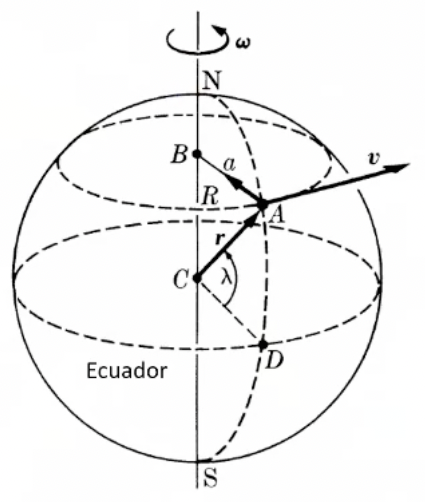
\includegraphics[width=0.25\textwidth]{problema_6.png}
\end{center}
\end{wrapfigure}


\textbf{Formulas base:}\\0

Se tomarán las siguientes formulas base del MCUA:

\begin{align}
\boxed{ \vec{a_{c}} = \frac{v^2}{r} = \frac{(w \cdot r)^2}{r} = w^2 \cdot r}\\
\boxed{ T = \frac{2\pi}{\omega}}\\
\boxed{ cos \lambda = \frac{R}{R_{T}}}
\end{align}

\textbf{Solución:}\\

Primero es necesario establecer algunas magnitudes conforme el SI, a saber:

\begin{align*}
T = 24\,h \cdot \frac{60\,m}{1\,h} \cdot \frac{60\,s}{1\,m} = 86400\,s\\
r = 6378.137\,k \cdot \frac{1000\,m}{1\,k} = 6378137\,m
\end{align*}

1. Para hallar la velocidad angular $\omega$, despejamos en la formula:

\begin{align}
\omega &= \frac{2 \cdot \pi}{24\,h} =  \frac{2 \cdot \pi}{86400\,s}  = 7.2722 \times 10^{-5} rad/s
\end{align}

2. Para hallar la velocidad lineal, es necesario deteminar el radio de giro (R) en función de la latitud (donde $R_{T}$ es el radio de la tierra), a saber:

\begin{align}
R &= R_{T} \cdot cos\,\lambda\\
R &= 6378137 \cdot cos\,\lambda
\end{align}

Ahora ya se puede despejar la velocidad, de la forma:

\begin{align}
V_{L} &= \omega \cdot R = 7.2722 \times 10^{-5} \cdot 6378137 \cdot cos\,\lambda\\ 
V_{L} &= 463.831\cdot cos\,\lambda\,m/s
\end{align}

3. Para determinar la aceleración centrípeta ($a_{c}$) en función de la latitud, se establece que:

\begin{align}
a_{c} = \frac{V_{L}^2}{r} = \frac{463.831 \cdot cos \lambda^2}{6378137 \cdot cos \lambda}\\
a_{c} = 3.3731 \times 10^{-2} \cdot cos \lambda\,m/s^2
\end{align}

En este punto, determinar donde pesa mas una persona, si en el ecuador o en el polo, esta sujeto al valor ángulo $\lambda$ y como este valor afecta la magnitud de la $a_{c}$ a saber:

\begin{align*}	
Si\,\lambda &= 0 \Rightarrow cos \lambda = 0\,(Ecuador)\\
Si\,\lambda &= 1 \Rightarrow cos \lambda = 1\,(Polo)
\end{align*}

Por lo que lo que la $a = a_{c} - g$ podrá tener dos valores diferentes, según donde se encuentre el observador, asi:

\begin{align*}	
Si\,\lambda &= 0 \Rightarrow a = 3.3731 \times 10^{-2} - 9.8 = - 9.77\,m/s^2\\
Si\,\lambda &= 1 \Rightarrow a = 0 - 9.8 = 9.8\,m/s^2
\end{align*}

Así que será en el Polo donde una persona pese mas, dado que será allí donde solo este presente la gravedad terrestre sin tener una afectación por la aceleración centrípeta.\\

4. Al comparar la gravedad presente en el Ecuador con la gravedad terrestre, se puede determinar la siguiente relación:

\begin{align*}	
\frac{g_{e}}{g_{t}} = \frac{9.77}{9.8} = 0.99
\end{align*}

Por lo que podemos concluir, que la $g_{e}$ es 0.99 veces la $g_{t}$.

%%%%%%%%%%%%%%%%%%%%

\end{document}

